\section{Designing the LUC-OS}
\label{sec:lucos}

% - Distributed clouds : hundreds micro DCs, which are themselves composed of up
%   to tens of servers 
% - Managing a distributed cloud -> managing thousands of geographically spread 
%   hosts.
% - P2P file sharing systems: example of software that works well in similar
%   conditions.
% - We think the file sharing systems should be an inspiration for the LUC-OS
%   design.
The massively distributed cloud we target, is an infrastructure that is composed
of up to hundreds of micro DCs, which are themselves composed of up to tens of 
servers, thus operating such an infrastructure means managing up to thousands of
geographically spread servers. Designing software that works at this scale is a
tedious task, as it comes with challenges such as preserving a good reactivity
(some operations should be performed as fast as possible) and implementing 
working fault tolerance mechanisms. Peer to peer file sharing systems (popular 
over the last decade) are a good example of software that works well at large 
scale in a context where computing resources are geographically spread. That is 
why we propose to learn from the experience of large scale peer to peer systems:
design rules of the LUC-OS architecture will be directly inspired by them. 

% - LUC-OS: distributed system: workload divided among every peers.
% - LUC-OS is a multi-agent system: each server (node) of the infrastructure 
%   host one LUC-OS agent.
% - A LUC-OS agent is composed of several services, each service is specialized
%   in a particular task.
% - To prevent bottlenecks and single point of failure, each service is 
%   distributed in a fully distributed manner: 
%    * bottleneck: in case a service is overloaded, it must be able to balance
%      workload on remote service instance.
%    * single point of failure: at large scale, failure becomes the norm rather
%      than the exception, services must implement self healing mechanisms and
%      each persistent state is stored in fault tolerant data structure (DHT).
% - To maximize the reactivity of the LUC-OS, a service should prioritize 
%   collaboration with corresponding services hosted on servers accessible with
%   low latency.
% - To enable low-latency collaborations, each service will leverage a locality
%   based overlay that will dynamically maintain for each server a list of 
%   neighbors.
The LUC-OS targets a fully distributed functioning inspired by the peer to peer
paradigm : its workload will be allocated over among every element constituting
the infrastructure. As we are interested by adding advanced properties 
(self-organization and self-healing) to the LUC-OS, we propose to leverage a 
multi-agent architecture: each node (server) constituting the infrastructure 
will host one of the LUC-OS agent. To prevent negative phenomenons such as
bottlenecks and single points of failure (SPOF), we have decided to anticipate
them during the design stage:

\begin{description}

  \item [Bottlenecks] : are caused by an excessive workload allocated to one 
  service, which slows its interactions with collaborators, thus impacting
  negatively the performance of the infrastructure by reducing both reactivity 
  and quality of service (QoS). Indeed, to prevent the overloading of a service,
  it is possible to distribute its workload on several underloaded remote 
  instances once the overload has occurred, or to take a proactive approach by 
  designing the service in a way that prevents overloading to happen.

  \item [Single points of failure] (SPOF) represents an element of a system, 
  that in case of failure, stops the entire system. As at large scale, failure 
  becomes the norm rather than the exception, SPOFs are a major concern in
  distributed software: that is why services must implement self healing 
  mechanisms such as redundancy. In addition each persistent state have to be 
  stored in fault tolerant data structure.

\end{description}

Before going into the details of the LUC-OS architecture, we give in Section
\ref{sec:ve} and \ref{sec:lbo} some definitions of some key concepts that are 
fundamental to the LUC-OS.

\subsection{Virtual environments}
\label{sec:ve}

% - Ressource allocation -> group of VMs.
% - Interconnection though virtual environment (VE).
% - specific requirement (hardware, placement) -> VE's constraint
% - Challenge: managing VEs in a fully distributed manner (p2p): 
%    -> ex of vm placement
The reference architecture exposed in Section \ref{sec:moreno} proposes a Cloud 
OS that enables users to create VMs that are interconnected by a network. As 
they are are tightly coupled, we think that VMs and their networks are parts
of a larger concept: the Virtual Environment (VE). In the same way that a 
desktop OS runs programs composed of threads, the Cloud OS will run VEs composed
of VMs. This analogy goes even further: in the same way threads are scheduled by
a desktop OS and thus can be executed by different CPUs in their life, a Cloud 
OS schedules VMs that may be migrated on different compute nodes. Thus the 
LUC-OS will enable its users to request the creation of groups of VMs 
interconnected in a VE though the use of a virtual network. Users may have 
specific requirements in terms of hardware and placement: this will result in 
constraints that will be integrated to the VE. Designing the LUC-OS raises the 
problem of managing VEs in a fully distributed manner: as the effort of hosting 
VEs will be spread over several LUC-OS nodes, thus some mechanisms that 
constitute IaaS needs to be revisited. For instance, VMs placement is typically 
decided by centralized service nodes, while there exists Distributed scheduling 
strategies such as DMVS \cite{quesnel:ispa2013} and 
\cite{DBLP:conf/cloudcom/FellerME12}. Related to the former point, when a VM is 
relocated on another LUC-OS node, the node should now take part its VE by 
sharing the hosting effort in terms of computing resources, networking and 
storage. Furthermore, the LUC-OS will provide advanced mechanisms that keep VMs
interconnectivity during hot relocations of VEs throughout distinct network 
domains.


\subsection{Overlay Networks and Locality}
\label{sec:lbo}

% - Overlay network -> logical network build on top of another networks.
% - abstraction for networking things (routing, lookup, fault tolerance).
% - LUC-OS will leverage this LBO and thus take full advantage of reactive 
%   inter-agent collaborations.
An overlay network is a logical network build on top of another physical or 
logical network, which enables to abstract networking things such as routing, 
lookup retrieval, and fault tolerance. One of the downsides of using overlay 
networks is that they break the physical topology by connecting nodes that have 
no physical proximity, thus potentially leading to an inefficient usage of the
network capabilities. In \cite{pastor:hal-00991530} authors proposed a Locality 
Based Overlay Network (LBO) that leverages Vivaldi \cite{dabek:2004:vivaldi}: an
algorithm which can provides dynamic coordinates to each node of the system, 
according to their respective latencies. Each node 
maintains a list of close contacts that are periodically and randomly exchanged.
This enables to build a distributed map of the infrastructure. The LBO enables 
high level applications to be aware of locality properties and thus to organize 
inter-agent collaborations in a way that minimize the network overhead and that 
improve the overall reactivity. The LUC-OS will also leverage overlay networks
such as the LBO to benefits from reactive inter-agent collaborations and from 
the capability delivered by the physical network infrastructure.





\subsection{Anatomy of a LUC-OS agent}

% - Figure \ref{fig:anatomy} -> our choices
% - 4 services: one service per aspect (compute, network, persistance, admin). 
% - Compute service: delivery of computing resources: built on top of:
%    * VMs broker: receives VM creation request, elect a server: it instantiate 
%      the VM; ensures VM creation.
%    * VMs scheduler: ensures good QoS for VMs: compute node overloaded ->
%      sched balances workload on underloaded ones (dynamic scheduling).
% - Network service: create virtual that interconnect VMs (broker). Network 
%   creation abstracted by the use network drivers (OpenFlow, Mininet, ...).
% - As some services manipulate hardware -> direct access via Hardware Drivers.
% - Persistence service: store states manipulated by the services of the LUC-OS:
%    * Objects (serializable entities); VMs images (VMs template) belonging to a 
%      specific user (+ metadata); VMs snapshots: like VM images with versions.
% - These sub-services leverage a DHT, and some of them leverage a resilient 
%   distributed FS.
% - Administrative: managing the infrastructure and producing statistical and 
%   usage data.
% - To perform those tasks it will leverage a DHT and a service that store 
%   execution logs of the infrastructure.

\label{sec:anatomy_lucos}
Figure \ref{fig:anatomy} depicts our architectural choices: each aspect of the 
LUC-OS is managed by a specific service that will collaborate with close 
instances of the service located on remote nodes through the use of locality
based network overlay. 

\subsubsection{Compute service}
is in charge of the delivery of computing power: it is built on top of two 
sub-services : \emph{VEs Spawner} is responsible for VEs creations and 
configurations and \emph{VMs Scheduler} guarantees a good QoS by performing 
dynamic scheduling. While these tasks are typically performed by centralized 
service nodes (OpenStack's Nova service), the LUC-OS take up the challenge of 
doing them in a fully distributed manner. This service covers features described
for \emph{Virtual machines manager} and \emph{Scheduler} in Section 
\ref{sec:moreno}.

\begin{figure*}
  \centerline{
   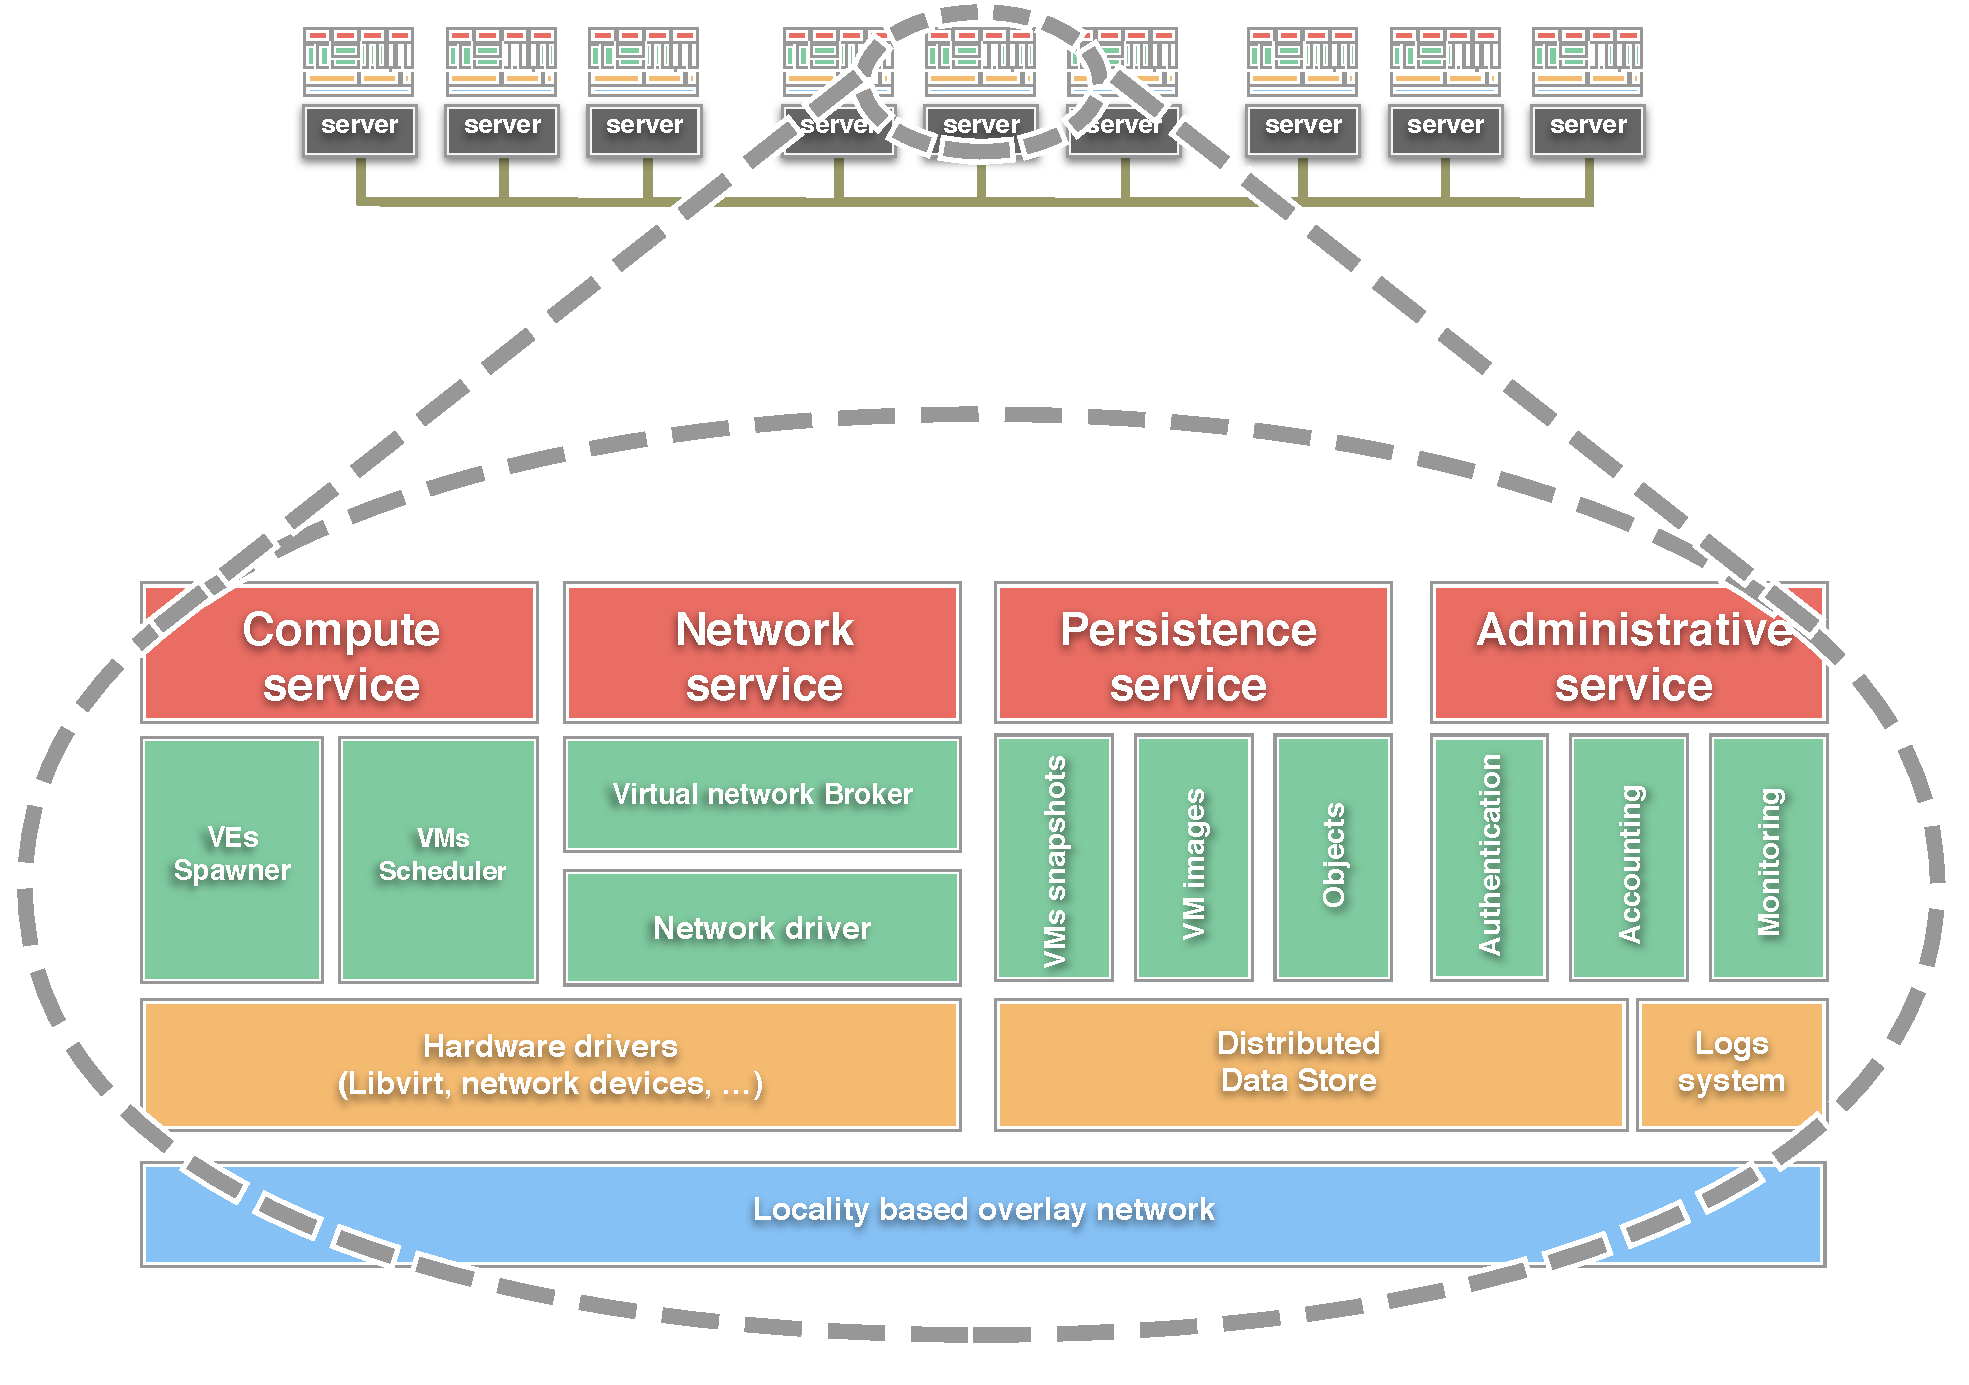
\includegraphics[width=1.55\linewidth]{Figures/lucos_agents.pdf}
  }
  \caption{Anatomy of services composing the LUC-OS.}%
  \label{fig:anatomy}%
  %\vspace*{-.8cm}
\end{figure*}

\subsubsection{Network service} 
leverages a \emph{Virtual Network Broker} that create virtual networks 
interconnecting VMs. Creation of these virtual networks is abstracted by the use
of \emph{Networking drivers}: it enables the use of a wide range of network 
technology such as OpenFlow \cite{McKeown:2008:OEI:1355734.1355746} and Mininet
\cite{Lantz:2010:NLR:1868447.1868466}. As all services composing Compute 
service and network drivers manipulate hardware, they will have direct access to
hardware via Hardware Drivers. This block must be able to maintain 
interconnectivity inside a VE, during the migration on distinct network domains 
of some of its VMs. This service covers features described for \emph{Network 
manager} in Section \ref{sec:moreno}.

\subsubsection{Persistence service}
is dedicated to keeping states of the LUC-OS by leveraging one service for each
kind of state: \emph{Objects} are used to persist serializable entities 
manipulated by the LUC-OS, \emph{VMs Images} are used for VMs template files 
(which belong to a specific user), \emph{VMs Snapshots} are pretty much the same
as VM images except that they support versionning. All the sub-services that 
compose the Persistence service leverage a \emph{Distributed Data Store}.As at 
large scale, failure becomes the norm rather than the exception, this service 
will rely on fault tolerant mechanisms that ensure the availability of stored 
resources in case of nodes failures. This service covers features of \emph{Image
manager} and \emph{Storage manager}, as described in Section \ref{sec:moreno}.

\subsubsection{Administrative service} 
will perform tasks such as managing the infrastructure and producing statistical
and usage data. To perform those tasks it will leverage the \emph{Distributed 
Data Store} and a service that stores execution logs of the infrastructure. The 
main challenge is to give the ability to users to manage their VEs from any 
LUC-OS agent, whether it is sharing its VEs hosting effort or not. This service 
covers features of \emph{Administrative tools} and \emph{Information manager,
Accounting/auditing}, as described in Section \ref{sec:moreno}.



